\documentclass[11pt,a4paper]{report}

\usepackage{graphicx,amsmath,amssymb,subfigure,url,xspace,textcomp,booktabs,siunitx,
  todonotes}
\usepackage{hyperref}
\usepackage[utf8]{inputenc}
\usepackage[bf]{caption}
\usepackage[
backend=bibtex,
style=numeric,
natbib=true,
url=true,
doi=true,
eprint=false
]{biblatex}

\addbibresource{../sources.bib}

\newcommand{\eg}{e.g.,\xspace}
\newcommand{\bigeg}{E.g.,\xspace}
\newcommand{\etal}{\textit{et~al.\xspace}}
\newcommand{\etc}{etc.\@\xspace}
\newcommand{\ie}{i.e.,\xspace}
\newcommand{\bigie}{I.e.,\xspace}


\title{Measurement of electrical properties (current-voltage and capacitance-voltage) of irradiated and non-irradiated silicon detectors}
\author{Michael Larson, Elisabeth Unger, Samuel Flis, Christian Bourjau}

\begin{document}
\maketitle

\section*{Introduction}
\label{sec:introduction}

Semiconductor sensors are omnipresent in the field of particle physics.
They are also deployed in areas exhibiting a large dose of radiation like the inner tracking systems of collider based experiments.
Therefore, it is crucial to understand the electrical properties and the response to radiation of these kind of detectors.
This laboratory exercise explores the  properties of Silicon (Si) based sensors by measuring the current and capacitance of these devices as a function of the applied reverse bias.
These measurements allow us to determine the depletion voltage of the given samples as well as to qualitatively observe the effect of radiation.

Applying and increasing a reverse voltage to a diode will lead to a growing depletion region until free charge carriers are absent in the entire volume of a pn-junction.
Hence, the at this point fully depleted volume works as an insulator in an electric field. The full depletion voltage $V_{fd}$ depends on the geometry and material of the diode and is given by 

\begin{equation}
  \label{Vfd}
  V_{fd} = \frac{q ~ N_{eff} ~ d^2}{2 ~ \epsilon_0 ~ \epsilon_r}
\end{equation}

where $q$ is the elementary charge ($\SI{1.6e-19}{C}$), $N_{eff}$ is the effective charge density at the boundary of the depleted region, $d$ is the length of the depleted region and $\epsilon_0 = \SI{8.85e-12}{F/m}$ is the vacuum permittivity and $\epsilon_r$ is the permittivity of the material in the depleted region ($\epsilon_r^{Si} = 11.68$)\cite{cv_iv_manual}.
The depleted region represents the active volume used for detection and its size $d$ can be deduced by rearranging \eqref{Vfd}.
Furthermore, the presence of two oppositely charged surfaces separated by an insulator provides the geometry of a parallel plate capacitor. Thus, the capacitance of the depleted diode can be expressed, using \eqref{Vfd}, as

\begin{equation}
  \label{C}
  C = \frac{\epsilon_{0} ~ \epsilon_{r} ~ A}{d}
\end{equation}

where $A$ is the area of one of the boundaries of the depleted region. Since the capacitance is governed by the size $d$ it will only increase with the applied voltage $V$ until the diode is fully depleted. For $V \geq V_{fd}$, the capacitance of the diode is given by

\begin{equation}
  \label{eq:1}
   C_{fd} = A ~ \sqrt{\frac{\epsilon_0 ~ \epsilon_r ~q ~ N_{eff}}{2 ~ V}}
\end{equation}

However, due to thermal excitations within the depleted region, a leakage current $I(V)$ is present whenever a voltage is applied to the diode.
At full depletion, the leakage current only depends on the rate at which electron-hole pairs are generated. Thus, $I(V)$ exhibits a plateau for $V>V_{fd}$.


\section*{Samples and measurement}
\label{sec:samples}

During this exercise, the current-voltage and capacitance-voltage relation of three different diodes were studied. While all samples were Silicon based, they differed in the type of doping used in their bulk region and in their exposure to radiation.
Presented here are the measurements of a non-irradiated p-type diode, a non-irradiated n-type diode and a second n-type diode irradiated by synchrotron radiation. 

The measurements were conducted in a clean room environment. The connections to the anode and cathode of each diode were achieved by placing a probe needle onto the sample.
A reverse bias was applied.
Furthermore, the experiment was shielded from light to avoid charge build-up due to the photoelectric effect. Subsequently, the current and capacitance of the diodes were measured over a range of different voltages. Each measurement was repeated three times in order to minimize statistical fluctuations and to investigate the systematic error of the experimental setup.

The diodes were scanned over a limited voltage range in order to avoid the creation of an avalanche discharge due to a thermal electron-hole pair.


\section*{Results}

In figure \ref{fig:cv} the diodes' inverse squared capacitance, $\frac{1}{C^{-2}}$ and the applied voltage $V$ is displayed.
A plateau of $1/C^2$ can be observed for all three diodes.
However, large deviations between the successive measurements were observed for the p-typed diode. These might have been caused by residual charges slowly draining in between successive measurements.
Discussions with more experienced colleagues indicated that the equipment has known inaccuracies when measuring small capacitances of order of $\sim pF$. Therefore the absolute scale of the capacitance cannot be relied upon, but the shape is reproducible between different measurements.
The full depletion voltage is estimated by fitting linear functions to the rising and plateaued regions. 

The intersection of the two functions is defined as the full depletion voltage $V_{fd}$.
Under this definition, it becomes clear that the radiation damage of the n-doped diode causes an increase of $V_{fd}$ from $25.16\pm0.20$ V (not irradiated) to $63.04\pm2.90$ V (irradiated).

% \begin{table}[]
% %\centering
% \caption{Summary of the results obtained from the CV and IV measurements.}
% \begin{tabular}{lllll}
% \toprule
% Sample type         & \multicolumn{2}{l}{Undepleted Region} & \multicolumn{2}{l}{Depleted Region}                                                          \\
%                     & Slope ($10^{-6}pF^{-2}V^{-1}$)        & Intercept ($10^{-3}pF^{-2}$) & Slope ($10^{-6}pF^{-2}V^{-1}$) & Intercept ($10^{-3}pF^{-2}$) \\
% \midrule
% P-Type              & 7.7$\pm$4.6                           & 37.3$\pm$0.8                 & 441.9$\pm$23.5                 & 5.0$\pm$0.3                  \\
% N-Type              & 22.6$\pm$4.9                          & 7.3$\pm$0.4                  & 171.7$\pm$2.7                  & -2.1$\pm$0.1                 \\
% N-Type (Irradiated) & 12.4$\pm$37.5                         & 58.0$\pm$3.0                 & 1978.6$\pm$110.3               &                              \\
% \bottomrule
% \end{tabular}
% \end{table}

\begin{table}
  \caption{Summary of measured values at the point of full depletion. The capacity is not shown since the absolute value proved to be unreliable.}\label{tab:results}
  \centering
  \begin{tabular}{lll}
    \toprule
    Sample type         & $V_{fd}$                 & $I(V_{fd})$ \\
    \midrule
    P-type              & $74.4 \pm 2.1 \si{V}$   &           \\
    N-type              & $25.2 \pm 0.2 \si{V}$  &             \\
    N-type (irradiated) & $63.0 \pm 2.9 \si{V}$ &             \\
    \bottomrule
  \end{tabular}
\end{table}



\label{sec:results}
\begin{figure}
  \centering
  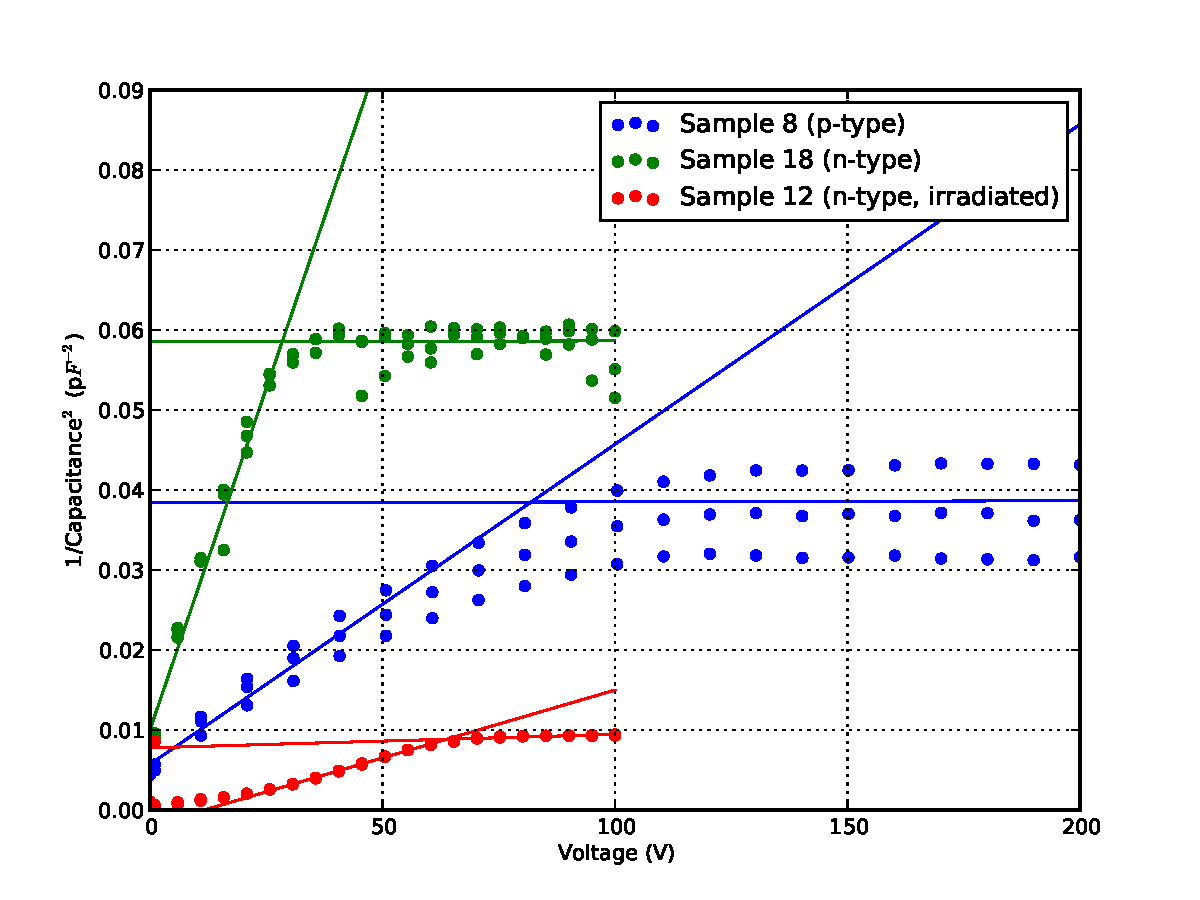
\includegraphics[width=0.8\textwidth]{./figures/cv.pdf}  
  \caption{Capacitance $C$ vs.\ applied voltage $V$ for the three studied samples. Each sample was measured three times. Note that the absolute values of the capacitance proofed to be unreliable in between consecutive measurements. The full depletion voltage $V_{fd}$ was unaffected by this circumstance and was specified by the intersection point of the linear fits of the rising and the plateaued region.}\label{fig:cv}
\end{figure}

Figure~\ref{fig:iv} shows the diodes' $I$-$V$ curves where the shaded area represent the spread observed in the three measurements.
The voltage ranges are identical with the ones used in the $C$-$V$ measurement.
The flattening of the current $I$ for $V>V_{fd}$ can be seen clearly in the n-doped samples.
Furthermore, the effect of the radiation damage is striking: The leakage current increased by about three orders of magnitude compared to the non-irradiated n-typed diode.
The results for $V_{fd}$ and $I(V_{fd})$  are summarized in table~\ref{tab:results}.

\begin{figure}
  \centering
  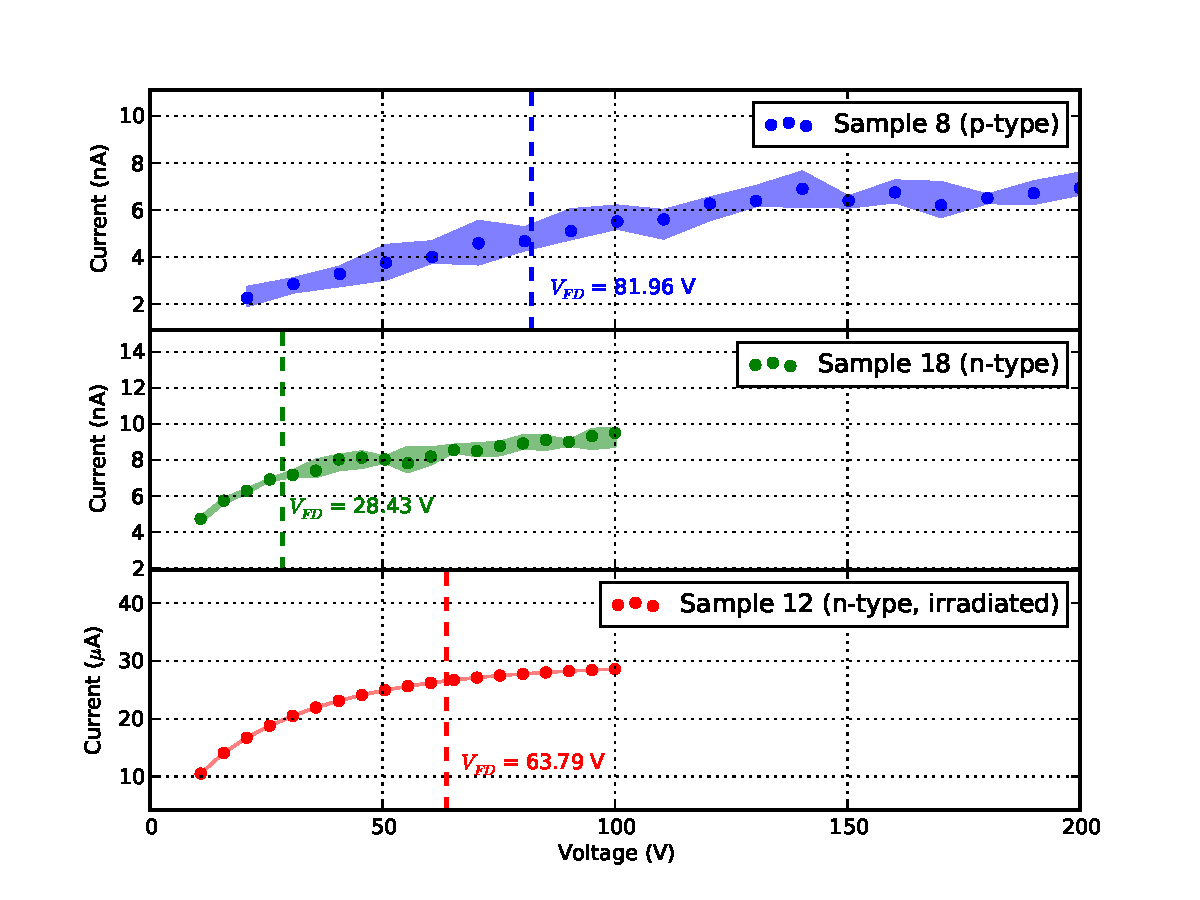
\includegraphics[width=0.8\textwidth]{./figures/iv.pdf}
  \caption{Current $I$ vs.\ applied voltage $V$ for the three studied samples. The depletion point $V_{fd}$ as extracted from the capacity-voltage measurement is depicted with the dashed line. Note the significantly higher current in case of the radiated sample.}\label{fig:iv}
\end{figure}



\section*{Summary}
\label{sec:summary}

The $C$-$V$ and $I$-$V$ curves of three different diodes were successfully measured.
While the scale of the capacitance $C$ was found to not be reliable, their shapes were reproducible in repeated measurements.
Based on these shapes it was possible to determine the full depletion voltage $V_{fd}$ for each diode and to observe the plateau in both curves for $V>V_{fd}$.
Radiation damage was found to cause an increase in $V_{fd}$ by a factor of $\sim 3$ and of the leakage current $I$ by three orders of magnitude.
This significant increase of the leakage current causes a deterioration of the signal-to-noise ratio in particle detectors.

\printbibliography

\end{document}

%%% Local Variables:
%%% mode: latex
%%% TeX-master: t
%%% End:
